\documentclass[tikz,border=10pt]{standalone}
\usepackage{tikz}
\usetikzlibrary{shapes.geometric, shapes.multipart, arrows.meta, positioning, calc, fit, backgrounds, shadows, patterns}

% Define colors to match
\definecolor{blue}{RGB}{0,0,255}
\definecolor{green}{RGB}{0,128,0}
\definecolor{yellow}{RGB}{255,255,0}
\definecolor{red}{RGB}{255,0,0}
\definecolor{orange}{RGB}{255,165,0}
\definecolor{gray}{RGB}{128,128,128}

\begin{document}
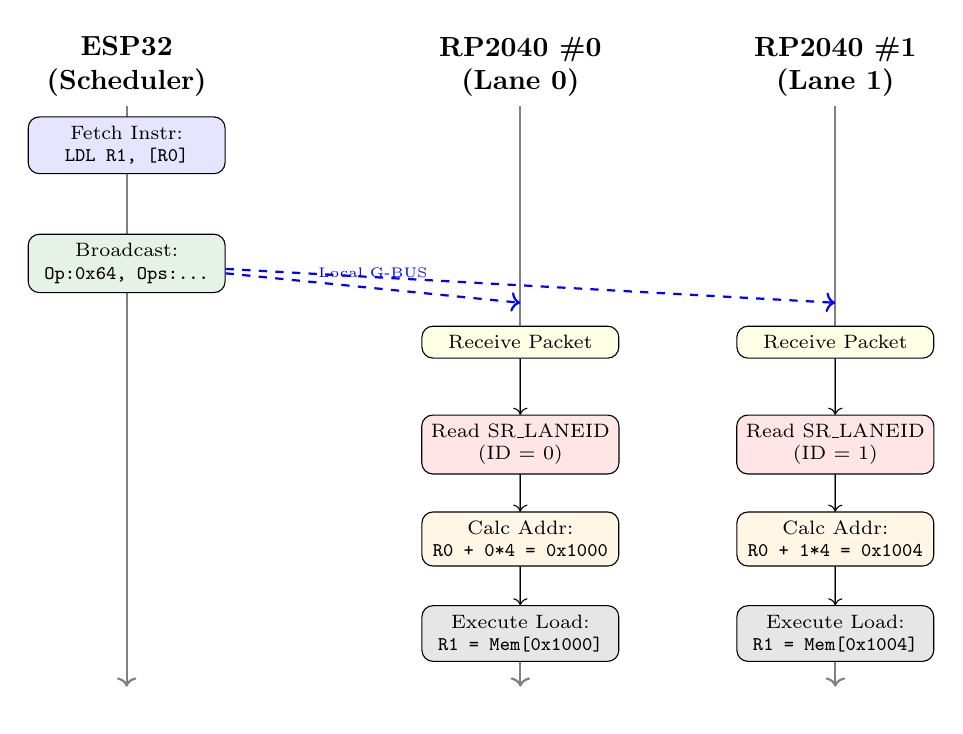
\begin{tikzpicture}[node distance=1.5cm, auto,
    timeline/.style={->, thick, gray},
    msg/.style={->, thick, blue, dashed},
    box/.style={rectangle, draw, fill=white, rounded corners, font=\scriptsize, align=center, minimum width=2.5cm}]

    % Timelines
    \node[align=center, font=\bfseries] (esp) at (0,0) {ESP32\\(Scheduler)};
    \node[align=center, font=\bfseries] (rp0) at (5,0) {RP2040 \#0\\(Lane 0)};
    \node[align=center, font=\bfseries] (rp1) at (9,0) {RP2040 \#1\\(Lane 1)};
    
    \node (esp_bot) at (0,-8) {};
    \node (rp0_bot) at (5,-8) {};
    \node (rp1_bot) at (9,-8) {};

    \draw[timeline] (esp) -- (esp_bot);
    \draw[timeline] (rp0) -- (rp0_bot);
    \draw[timeline] (rp1) -- (rp1_bot);

    % Events
    \node[box, fill=blue!10] (fetch) at (0, -1) {Fetch Instr:\\\texttt{LDL R1, [R0]}};
    \node[box, fill=green!10] (broadcast) at (0, -2.5) {Broadcast:\\\texttt{Op:0x64, Ops:...}};

    \draw[msg] (broadcast) -- node[above, font=\tiny] {Local G-BUS} (5, -3);
    \draw[msg] (broadcast) -- (9, -3);

    % RP2040 Processing
    \node[box, fill=yellow!10] (rx0) at (5, -3.5) {Receive Packet};
    \node[box, fill=yellow!10] (rx1) at (9, -3.5) {Receive Packet};

    \node[box, fill=red!10] (lane0) at (5, -4.8) {Read SR\_LANEID\\(ID = 0)};
    \node[box, fill=red!10] (lane1) at (9, -4.8) {Read SR\_LANEID\\(ID = 1)};

    \draw[->] (rx0) -- (lane0);
    \draw[->] (rx1) -- (lane1);
    
    \node[box, fill=orange!10] (addr0) at (5, -6.0) {Calc Addr:\\\texttt{R0 + 0*4 = 0x1000}};
    \node[box, fill=orange!10] (addr1) at (9, -6.0) {Calc Addr:\\\texttt{R0 + 1*4 = 0x1004}};

    \draw[->] (lane0) -- (addr0);
    \draw[->] (lane1) -- (addr1);

    \node[box, fill=gray!20] (load0) at (5, -7.2) {Execute Load:\\\texttt{R1 = Mem[0x1000]}};
    \node[box, fill=gray!20] (load1) at (9, -7.2) {Execute Load:\\\texttt{R1 = Mem[0x1004]}};

    \draw[->] (addr0) -- (load0);
    \draw[->] (addr1) -- (load1);

\end{tikzpicture}
\end{document}
